% ============================================================================
% Budget-Agnostic UAP Deployment -- ACM ASIACCS 2027 (Cycle 2) submission
% Format: ACM Primary Article Template, sigconf, double-column, double-blind.
% Compile on Overleaf: pdfLaTeX, run twice. Requires the acmart class
% (Overleaf: Menu -> Settings -> TeX Live version 2023+ ships acmart).
% Body text target: <= 12 pages excluding bibliography and appendices.
% NOTE: every numeric cell in tables/ is auto-generated from the result JSONs
% by make_tables.py -- never hand-edit numbers.
% ============================================================================
% `nonatbib`: the reference list is a hand-written thebibliography with plain
% \bibitem entries, which natbib's default author-year mode would reject
% ("Bibliography not compatible with author-year citations"). Only \cite is
% used, so plain numeric citations are what we want.
\documentclass[sigconf,anonymous,review,nonatbib]{acmart}

% acmart already pulls in booktabs, xcolor, graphicx, hyperref and -- through
% newtxmath -- amsmath. Two rules follow from that:
%   * nothing the class already provides is loaded a second time;
%   * amssymb must NOT be loaded at all. acmart's font setup calls newtxmath,
%     which already defines \Bbbk; the TeX Live 2025/2026 amssymb then aborts
%     with "Command \Bbbk already defined" at amssymb.sty line 261.
% The only amssymb symbols used by this paper are \mathbb (provided by
% newtxmath) and a QED tombstone, which is defined below with rules instead.
\makeatletter
\@ifpackageloaded{booktabs}{\relax}{\usepackage{booktabs}}
\@ifpackageloaded{amsmath}{\relax}{\usepackage{amsmath}}
\@ifpackageloaded{algorithm}{\relax}{\usepackage{algorithm}}
\@ifpackageloaded{algorithmic}{\relax}{\usepackage{algorithmic}}
\@ifpackageloaded{xcolor}{\relax}{\usepackage{xcolor}}
\makeatother

% Font-independent end-of-proof box (same shape as amsthm's \openbox).
\providecommand{\openbox}{\leavevmode
  \hbox to.77778em{\hfil\vrule\vbox to.675em{\hrule width.6em\vfil\hrule}\vrule\hfil}}

\providecommand{\eps}{\ensuremath{\epsilon}}
\providecommand{\sat}{\mathrm{sat}}
\providecommand{\todo}[1]{\textcolor{red}{[TODO: #1]}}

% Float placement: this paper carries 12 full-width tables and 3 full-width
% figures; loosen the default limits so they are not deferred to the end.
\setcounter{topnumber}{3}
\setcounter{totalnumber}{4}
\renewcommand{\topfraction}{0.92}
\renewcommand{\textfraction}{0.06}
\renewcommand{\floatpagefraction}{0.75}

\acmConference[AsiaCCS '27]{ACM Asia Conference on Computer and Communications Security}{July 12--16, 2027}{Macau, China}
\acmYear{2027}

\begin{document}

\title{Train Once, Deploy at Any Budget: Budget-Agnostic Deployment of
Universal Adversarial Perturbations}

\author{Anonymous Author(s)}
\affiliation{%
  \institution{Anonymous Institution}
  \city{Anonymous City}
  \country{Anonymous Country}
}

% ----------------------------------------------------------------------------
\begin{abstract}
Universal adversarial perturbations (UAPs) are typically trained and evaluated
at a single perturbation budget $\eps$. We show that this coupling is an
artifact of common practice, not a requirement: a UAP trained once at a small
budget $\eps_w$ can be \emph{linearly rescaled} to any larger budget with no
loss of fidelity, covering the entire budget range at a fraction of the
training cost. On ImageNet with 200 training images, our scale-up deployment
matches or exceeds per-budget retraining of the strongest modern baselines
(TSC-UAP, TIFS'24; DM-UAP, AAAI'25) at $\eps\ge 0.2$---and trails the best of
seven baselines spanning 2017--2025 by at most $1.4$\,pp at $\eps{=}0.1$---while
using $3.0\times$--$9.7\times$ less training compute; against DM-UAP---which we
deliberately grant $3.3\times$ more wall-clock per run---it matches or beats
DM-UAP at every budget: statistical parity at $\eps{=}0.1$
($-1.4$\,pp, n.s.) and a modest but significant advantage at $\eps\ge 0.2$
($+5.3$ and $+3.5$\,pp; $t{=}2.70$ and $4.04$). We
further give a
mechanistic account of \emph{when} budget-coupled training fails:
(i) under few-shot data, high-$\eps$ direct training yields poorly-structured
directions (\emph{undersaturation}), predicted by the saturation fraction
$\sat$; and (ii) the folklore alternative of training once at the largest
budget and \emph{clipping down} degrades fooling rate in proportion to the
quality of the underlying direction, not the amount clipped. A pre-registered
control on CIFAR-10, where every method, budget, and deployment strategy is
pinned to the same irreducible fooling-rate ceiling ($\approx$91\%), confirms
the advantage is conditioned on the ceiling being unbinding and vanishes in
the ceiling-bound regime. We position these results as a deployment primitive
and a diagnostic, and delineate five explicit boundaries of the claims.
\end{abstract}

% --- ACM metadata (required by the CFP: retain CCS concepts / keywords) -----
\ccsdesc[500]{Security and privacy~Software and application security}
\ccsdesc[300]{Computing methodologies~Machine learning}
\ccsdesc[100]{Theory of computation~Design and analysis of algorithms}

\keywords{universal adversarial perturbations, budget-agnostic deployment,
transferability, few-shot adversarial optimization, evaluation protocol}

\maketitle

% ----------------------------------------------------------------------------
\section{Introduction}

\textbf{P1 --- The coupling is convention, not necessity.}
Universal adversarial perturbations
(UAPs)~\cite{moosavi2017universal}---single perturbations that fool a
classifier on most inputs, in the broader family of adversarial
examples~\cite{szegedy2014intriguing,goodfellow2015fgsm,carlini2017cw}---are
trained one perturbation per budget in the entire literature. We propose
\emph{budget-agnostic deployment}: train once, deploy at any budget. The key
technical fact is that low-budget training followed by linear rescaling
(scale-up) is shape-preserving and lossless: the per-coordinate saturation
profile is invariant under scaling, and no projection is involved.

\textbf{P2 --- A counterintuitive empirical reversal.}
Under few-shot data ($k{=}200$), direct training at the target budget
(budget-coupled) is beaten badly by scale-up on ImageNet:
$+7.6$/$+19.2$/$+26.6$\,pp FR at $\eps{=}0.1/0.2/0.3$ (black-box mean over
three surrogates). The mechanism:
high-$\eps$ few-shot training is \emph{undersaturated}
($\sat$ drops $0.53 \to 0.03$), producing poorly-structured directions;
low-budget training is naturally saturated, and scaling preserves the shape.

\textbf{P3 --- Compute-aligned comparison against modern baselines.}
Under the same 200-shot protocol, scale-up-TSC covers all three budgets with
$1/3$ the compute of per-budget TSC retraining and $1/10$ of DM-UAP's
(DM-UAP receives $3.3\times$ more wall-clock per run): statistically equivalent to
TSC at all three budgets, parity with DM-UAP at $\eps{=}0.1$
($-1.4$\,pp, $t{=}-0.38$, n.s.), and a modest but significant advantage at
$\eps\ge 0.2$ ($+5.3$\,pp, $t{=}2.70$; $+3.5$\,pp, $t{=}4.04$).

\textbf{P4 --- Two mechanisms, two quantities.}
$\sat$ (fraction of saturated coordinates) explains why budget-coupled
training collapses; $\mathrm{clip\text{-}frac}$ (fraction of coordinates
clipped by clip-down) explains why the folklore clip-down strategy degrades
by amounts that vary $9\times$ across optimizers (at $\eps{=}0.1$: TSC,
$89\%$ of coordinates clipped, $-1.5$\,pp; SGD, $42\%$ clipped,
$-13.8$\,pp). The damage of clipping
lies in direction quality, not truncation amount.

\textbf{P5 --- Cross-dataset control and boundaries.}
On CIFAR-10 all four optimizers, budgets, and deployment strategies are
pinned to the same irreducible FR ceiling ($\approx$91\%); there the advantage
disappears ($|\Delta|\le 0.07$\,pp) even though an undersaturation gap is
still measurable---showing \emph{both} factors must hold, and the claims are
conditioned, not universal. Five explicit boundaries in \S\ref{sec:limits}.

\medskip
\noindent\textbf{Contributions.}
\begin{enumerate}
  \item A budget-agnostic deployment primitive: one training covers any
        budget at $3.0\times$--$9.7\times$ less compute than the baselines it
        matches, with black-box FR no
        worse than the TIFS'24 / AAAI'25 baselines at $\eps\ge 0.2$
        (conditioned claim);
  \item Two mechanistic quantities, $\sat$ and $\mathrm{clip\text{-}frac}$,
        that respectively explain budget-coupled failure and the
        optimizer-dependence of clip-down cost;
  \item A complete evidence chain over seven baselines (2017--2025) with a
        clip-down counterfactual and a pre-registered CIFAR-10
        ceiling-bound-regime control, including negative results.
\end{enumerate}

% ----------------------------------------------------------------------------
\section{Related Work}
\textbf{Adversarial examples.}
Adversarial examples were first observed by Szegedy et
al.~\cite{szegedy2014intriguing} and explained as gradient-linear behaviour by
the FGSM account~\cite{goodfellow2015fgsm}; strong iterative attacks followed,
including C\&W~\cite{carlini2017cw} and PGD~\cite{madry2018pgd}. Transfer to
unpublished models---the black-box setting we evaluate in---was established
by practical black-box attacks~\cite{papernot2017practical} and studied at
scale by Liu et al.~\cite{liu2017ndss}; physical-world instantiations include
stickers~\cite{evtimov2018semantic}. Universal perturbations
\cite{moosavi2017universal} compress this threat into a single
image-agnostic $\delta$.

\textbf{UAP: a data-usage spectrum.}
Since the original iterative boundary discovery~\cite{moosavi2017universal},
UAP methods span a spectrum of data requirements. At the low-data end,
(p,q)-singular vectors of layer Jacobians yield UAPs from as few as 64
images~\cite{khrulkov2018art}. Fully data-free methods optimize surrogate
objectives on random inputs: Fast Feature Fool~\cite{mopuri2017ffa} maximizes
multi-layer activation means, its journal successor generalizes the objective
across tasks~\cite{mopuri2019generalizable}, and generator networks output
perturbations in one forward pass~\cite{poursaeed2018generative}. Between the
ends, feature-disruption methods train from unlabeled or out-of-distribution
data~\cite{wang2024fduap}, and meta-learning targets transferable
\emph{targeted} UAPs~\cite{weng2024metauap}. A recent comparative
evaluation~\cite{weng2024survey} systematizes noise-based and
generator-based training. Our setting uses 200 labeled images but asks an
orthogonal question (below).

\textbf{Modern UAP.}
TSC-UAP~\cite{huang2024texture} constrains the texture scale of the
perturbation map and repeats it over the image domain, substantially
improving fooling rate and transfer; we use it both as a strong baseline and
as the optimizer inside our scale-up primitive. Feature-disruption
UAP~\cite{wang2024fduap} disrupts model-agnostic channel features for
transfer. DM-UAP~\cite{zhang2025dmuap} improves UAP generalization via
dynamic maximin optimization over model--data pairs; it is the strongest
modern baseline in our comparison. On the defense side, Akhtar et
al.~\cite{akhtar2018defense} detect and reconstruct UAP-perturbed inputs,
and universal adversarial training~\cite{shafahi2019universal} embeds the
UAP objective into robust training; neither touches the training--deployment
budget coupling.

\textbf{Data efficiency and our question.}
Data efficiency is a recognized axis: singular-vector UAPs operate from 64
images~\cite{khrulkov2018art}, data-free objectives from
none~\cite{mopuri2017ffa,mopuri2019generalizable,poursaeed2018generative},
meta-learning from a task distribution~\cite{weng2024metauap}. These works
ask \emph{how well} a UAP can be trained from little data. We ask whether
the training budget must equal the deployment budget \emph{at all}. To our
knowledge, no published work explicitly studies this training--deployment
decoupling.

\textbf{Budget practices in adversarial robustness.}
Multi-budget evaluation is the default reporting convention in adversarial
robustness: fixed $\eps$ grids in robust training~\cite{madry2018pgd},
attack evaluation~\cite{carlini2017cw,athalye2018obfuscated}, and
standardized benchmarks~\cite{croce2021robustbench}---yet every reported UAP
is trained \emph{at} the budget it is evaluated on. The coupling is
therefore a convention inherited from evaluation practice; our results show
it carries a real compute cost and can mask a training failure mode.

% ----------------------------------------------------------------------------
\section{Problem Setting and Threat Model}\label{sec:setting}
\textbf{UAP.} For classifier $f$ and data distribution $\mathcal{D}$, a UAP
\cite{moosavi2017universal} is
$\|\delta\|_\infty \le \eps$ maximizing the fooling rate
$\mathrm{FR}(\delta)=\Pr[f(x+\delta)\neq f(x)]$.
\textbf{Few-shot protocol.} The attacker sees $k{=}200$ training images
(fixed seed, disjoint from evaluation); evaluation uses 2{,}000 held-out
images on a 5-model matrix (ResNet-50/101~\cite{he2016resnet},
VGG-16-BN~\cite{simonyan2015vgg}, MobileNet-V2~\cite{howard2018mobilenet},
ViT-B/16~\cite{dosovitskiy2021vit}): white-box surrogate plus black-box
heterogeneous targets.
\textbf{Budgets.} $\eps\in\{0.1,0.2,0.3\}$ on $[0,1]$ pixels.
\textbf{CIFAR-10 control.} Same protocol with 8 CIFAR-10
architectures~\cite{krizhevsky2009cifar}
(ResNet-18/34/50/101~\cite{he2016resnet}, VGG-16-BN~\cite{simonyan2015vgg},
DenseNet-121~\cite{huang2017densenet}, MobileNet-V2~\cite{howard2018mobilenet},
ShuffleNet-V2~\cite{ma2018shufflenet}); surrogates \{ResNet-50, VGG-16-BN,
MobileNet-V2\}, targets = all non-surrogate models; identical train/eval
splits, seeds, and budgets.

% ----------------------------------------------------------------------------
\section{Budget-Agnostic Deployment}\label{sec:method}
\textbf{Scale-up primitive.} Train once at a warm-start budget
$\eps_w < \eps$: $\delta_w = \textsc{TrainOpt}(f, D_k, \eps_w)$; deploy
$\delta(\eps) = (\eps/\eps_w)\,\delta_w$ (Algorithm~\ref{alg:scaleup}).
Two properties (proved in Appendix~\ref{app:proof}):
(i) \emph{shape preservation}: $\|\delta(\eps)\|_\infty = \eps$ and the
per-coordinate boundary profile is invariant;
(ii) \emph{zero loss}: rescaling is an invertible radial bijection between
the $\eps_w$-ball and the $\eps$-ball; no projection, no truncation.
Empirically the invariance in (i) is visible in the CIFAR-10 control
($\sat(\delta(\eps))\equiv\sat(\delta_w)$ across all deployment budgets;
\S\ref{sec:exp}).

% The `algorithm` package provides no starred (full-width) float, so the
% pseudocode is written to fit a single 3.3in column of the sigconf layout.
\begin{algorithm}[t]
\caption{Budget-agnostic deployment (scale-up). One training run covers all
$B$ budgets; every deployed $\delta^{(j)}$ satisfies
$\|\delta^{(j)}\|_\infty=\eps^{(j)}$ by construction.}\label{alg:scaleup}
\begin{algorithmic}[1]
\REQUIRE $f$, pool $D_k$, warm start $\eps_w$,
  targets $\eps^{(1)}{<}\cdots{<}\eps^{(B)}$
\STATE $\delta_w \gets \textsc{TrainOpt}(f, D_k, \eps_w)$
\FOR{$j = 1$ to $B$}
  \STATE $\delta^{(j)} \gets (\eps^{(j)}/\eps_w)\,\delta_w$
\ENDFOR
\STATE \textbf{return} $\{\delta^{(1)},\dots,\delta^{(B)}\}$
\end{algorithmic}
\end{algorithm}
\textbf{Training-run alignment.} Covering $B$ budgets takes $B$ runs for
per-$\eps$ retraining but a single run for both scale-up and clip-down; all
comparisons respect this alignment.

% ----------------------------------------------------------------------------
\section{Why Budget-Coupled Training Fails: Two Mechanisms}\label{sec:mech}
\textbf{Mechanism 1 (undersaturation).} With few-shot data and fixed learning
rate, high-$\eps$ direct training has
$\sat(\delta;\eps)=\Pr[|\delta_i|\approx\eps]$ collapsing in $\eps$
(ResNet: $0.53\to0.03$); directions are ill-structured. Low-budget training is
naturally saturated and scaling preserves the profile. Two-factor criterion:
a positive gap $\Delta = \text{scale-up} - \text{direct}$ \emph{requires}
\emph{(a)} direct to be undersaturated (significant $\sat$ gap) \emph{and}
\emph{(b)} the FR ceiling not to be binding; when both hold we observe
$\Delta>0$ in $12/15$ dataset--pair cells, the three exceptions being exactly
the ceiling-hit models. Evidence: ImageNet (both factors)
$6/6$ strongly positive; CIFAR-10 (factor (b) absent: all strategies pinned
to a common $\approx$91\% ceiling) $|\Delta|\le 0.07$\,pp despite a measurable
undersaturation gap---establishing that the factors are individually
necessary. Across datasets Pearson $r=0.807$ ($n{=}15$, sign-consistent
$12/15$).

\medskip
\noindent\textbf{Interventional confirmation.}
Table~\ref{tab:ksweep} manipulates the proposed cause directly: holding the
optimizer, budget, and protocol fixed and enlarging the few-shot pool from
$k{=}200$ to $k{=}500$ restores direct training's saturation (at
$\epsilon{=}0.1$, $\sat$: $0.53\to0.91$) and collapses the scale-up
advantage from $+34$--$41$\,pp to ${\approx}1$\,pp; at $k{=}1000$ it is
indistinguishable from zero (all three seeds agree). The advantage is thus
an artifact of the named training regime, not of the deployment primitive:
remove the regime and the effect disappears, as the criterion predicts.
% AUTO-GENERATED by make_tables.py -- DO NOT EDIT
\begin{table}[t]\centering\small\setlength{\tabcolsep}{4pt}
\caption{Data-size sweep ($k{=}200/500/1000$, ResNet-50 surrogate, black-box mean over 3 seeds; per-seed patterns are identical). For each $k$ and $\epsilon$: direct-training fooling rate, its saturated-coordinate fraction $\sat$, and the gap $\Delta$ to scale-up. The intervention predicted by the two-factor criterion: as $k$ grows, $\sat$ rises ($0.53\to0.91$ at $\epsilon{=}0.1$) and the scale-up advantage collapses from $+34$--$41$\,pp to $\approx 1$\,pp.}
\label{tab:ksweep}
\begin{tabular}{lcccc}\toprule
$k$ & $\epsilon$ & direct FR & $\sat$ & $\Delta$ (pp) \\
\midrule
200 & 0.1 & 0.486 & 0.527 & +34.5 \\
200 & 0.2 & 0.574 & 0.135 & +36.5 \\
200 & 0.3 & 0.579 & 0.029 & +41.3 \\
\midrule
500 & 0.1 & 0.818 & 0.913 & +1.0 \\
500 & 0.2 & 0.935 & 0.777 & -0.3 \\
500 & 0.3 & 0.989 & 0.641 & +0.0 \\
\midrule
1000 & 0.1 & 0.821 & 0.925 & +0.9 \\
1000 & 0.2 & 0.934 & 0.809 & -0.6 \\
1000 & 0.3 & 0.990 & 0.665 & -0.2 \\
\bottomrule\end{tabular}\end{table}

\medskip
\noindent\textbf{Why undersaturation arises: a step-size--budget mismatch.}
\emph{Minimal model} (per-coordinate, decoupled): coordinate $i$ receives
independent aligned drift $\mu_i > 0$ with cdf $F_\mu$ and zero-mean noise
$\sigma\xi$, and is trained by projected gradient ascent with fixed step
size $\eta$ for $T$ steps from $\delta_0 = 0$:
$\delta_i^{t+1} = \Pi_{[-\eps,\eps]}\!\big(\delta_i^t +
\eta(\mu_i + \sigma\xi_i^t)\big)$.

\textbf{Proposition 1 (budget-coupled saturation collapse).}
In the drift-dominated regime, coordinate $i$ saturates iff
$\mu_i \ge \eps/(\eta T)$, so
$\sat(\eps) = 1 - F_\mu\!\big(\eps/(\eta T)\big)$:
the saturated fraction is non-increasing in $\eps$ and vanishes as $\eps$
grows, at fixed $(\eta, T)$---enlarging the budget \emph{mechanically}
produces an interior iterate (proof in Appendix~\ref{app:proof}). With
drift noise the threshold shifts per coordinate by $\eta\sigma\sqrt{T}z$
($z \sim \mathcal{N}(0,1)$), producing a noise floor. Figure~\ref{fig:theory}
shows the closed forms track simulated dynamics of this model
(mean absolute error $0.026$ over $25$ budgets).

\textbf{Proposition 2 (scale-up is exact).}
For any $\eps \ge \eps_w$, the rescaled perturbation satisfies
$\|\delta(\eps)\|_\infty \le \eps$ with
$\sat(\delta(\eps);\eps) = \sat(\delta_w;\eps_w)$ \emph{exactly, at every
budget}: saturation is invariant under rescaling and no coordinate is ever
truncated (proof in Appendix~\ref{app:proof}).

\textbf{Proposition 3 (clip-down collapses the profile).}
Scale-up preserves every cross-coordinate ratio
$\delta_i(\eps)/\delta_j(\eps) = \delta_{w,i}/\delta_{w,j}$; clip-down maps
every clipped coordinate to $\pm\eps$, collapsing the ratio structure on the
clipped set to a constant. Directional information therefore survives
rescaling exactly and is destroyed by truncation in proportion to the
clipped mass---the geometric content behind Mechanism~2
(proof in Appendix~\ref{app:proof}).

\emph{Scope.} The model is deliberately minimal (decoupled coordinates; no
coupling through the loss, network, or data). Its value is that the two
empirical signatures---$\sat$ collapsing in $\eps$ at fixed $(\eta,T)$
(Fig.~\ref{fig:theory}) and $\sat$ invariance under rescaling (observed
exactly in the CIFAR-10 control)---follow from the model in the same form
as observed, and that the data-size intervention of Table~\ref{tab:ksweep}
($k \uparrow \Rightarrow \mu$-mass rises above threshold $\Rightarrow$
advantage vanishes) manipulates precisely the quantity the model names.
\begin{figure*}[t]
\centering
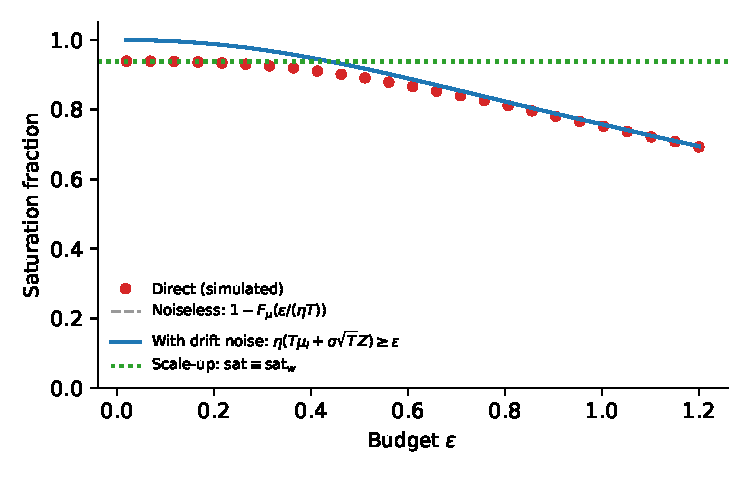
\includegraphics[width=.78\linewidth]{figs/theory_sat.pdf}
\caption{The minimal model of Proposition~1: saturation fraction versus
budget for direct projected gradient ascent (simulated, $n{=}20{,}000$
coordinates, lognormal drifts, $T{=}200$), the noiseless closed form
$1 - F_\mu(\eps/(\eta T))$, the drift-noise closed form, and the scale-up
level $\sat_w$ (Proposition~2), which is budget-invariant.}
\label{fig:theory}
\end{figure*}
\textbf{Mechanism 2 (direction quality governs clipping cost).} Clip-down
$\delta_{\downarrow} = \Pi_{\|\cdot\|_\infty\le\eps}(\delta_{\eps_{\max}})$ is
not explained by $\mathrm{clip\text{-}frac}$: at $\eps{=}0.1$ TSC loses
$1.5$\,pp with $89\%$ of coordinates clipped, a figure that is a partial
cancellation across surrogates ($-5.6$ ResNet-101, $-4.9$ ResNet-50, $+6.1$
ViT-B/16) and therefore unresolved, whereas SGD loses $13.8$\,pp relative to
scale-up with only $42\%$ clipped, and even $6.2$\,pp relative to honest
per-$\eps$ retraining. Clipping does not change directions; a bad direction
clipped is still bad.

% ----------------------------------------------------------------------------
\section{Experiments}\label{sec:exp}
\subsection{Setup}
Table~\ref{tab:protocol} summarizes the protocol. In eval mode the
evaluation batch size does not affect FR (batch-norm uses running
statistics); we verified this empirically before the main runs. All tables
and figures in this paper are generated programmatically from the released
result JSONs.
\begin{table*}[t]
\centering
\caption{Experimental protocol.}
\label{tab:protocol}
\small
\begin{tabular}{ll}
\toprule
Datasets & ImageNet-mini (train/val), CIFAR-10 (train/test) \\
Train / eval images & $k{=}200$ / 2{,}000 (disjoint, fixed seeds) \\
Model matrix (ImageNet) & ResNet-50/101, VGG-16-BN, MobileNet-V2, ViT-B/16 \\
Model matrix (CIFAR-10) & ResNet-18/34/50/101, VGG-16-BN, \\
 & DenseNet-121, MobileNet-V2, ShuffleNet-V2 \\
Surrogates (ImageNet) & ResNet-50, ResNet-101, ViT-B/16 \\
Surrogates (CIFAR-10) & ResNet-50, VGG-16-BN, MobileNet-V2 \\
Budgets $\eps$ & $0.1 / 0.2 / 0.3$ ($L_\infty$, $[0,1]$ pixels) \\
Warm-start $\eps_w$ / clip source $\eps_{\max}$ & $0.05$ / $0.3$ \\
Optimizers & SGD (lr 0.01, 200 steps), TSC, UAP'17, DM-UAP (official) \\
Seeds & $42, 1342, 2342$ \\
Metric & FR $=\Pr[f(x+\delta)\neq f(x)]$, black-box mean over targets \\
\bottomrule
\end{tabular}
\end{table*}

\subsection{Main comparison (ImageNet, 200-shot)}
Table~\ref{tab:main-imagenet}. Three readings. (1) Scale-up-TSC is the best
method at $\eps{=}0.3$ (99.2, ahead of every per-budget run) and statistically
indistinguishable from the best at $\eps{=}0.2$ (94.3 vs.\ TSC-UAP's 94.4,
$0.1$\,pp, far inside seed noise)---despite one training run; at $\eps{=}0.3$
it nominally edges out its own per-budget retraining (99.2 vs.\ 99.1,
$t{=}0.93$, n.s.). (2) At
$\eps{=}0.1$ DM-UAP leads; we state plainly that scale-up-SGD trails badly
there ($-16.5$\,pp, $t{=}-19.2$, $0\%$ positive), while scale-up-TSC is at
parity ($-1.4$\,pp, $t{=}-0.4$, n.s.). The $\eps{=}0.1$ regime is precisely where the
two-factor criterion predicts weak or no advantage---DM-UAP's dynamic
optimization keeps directions well-structured, leaving no undersaturation
gap for scale-up to exploit. (3) The ceiling row ($81.7$ at $\eps{=}0.1$)
compresses all differences; with one run, scale-up-TSC reaches
$96.1\%$/$99.4\%$/$100.3\%$ of the 2000-shot reference ceiling at
$\eps{=}0.1/0.2/0.3$. (This reference is itself a 2000-shot attack, not a
theoretical bound; at $\eps{=}0.3$ the two are within half a point, so the
ordering there is not meaningful.)
% AUTO-GENERATED by make_tables.py -- DO NOT EDIT BY HAND
\begin{table*}[t]
\centering
\caption{ImageNet: black-box fooling rate (\%) of one UAP shared across all transfer targets, mean over 3 surrogates $\times$ 3 seeds $\times$ heterogeneous targets (200-shot training data). Ceiling: 2000-shot multi-step reference attack (not a theoretical bound). DM-UAP receives $3.3\times$ more wall-clock per run (measured). Cells are rounded to one decimal, so a paired $\Delta$ quoted in the text can differ from the difference of two displayed cells by $0.1$\,pp.}
\label{tab:main-imagenet}
\small
\begin{tabular}{lcccc}
\toprule
Method & Train runs & $\epsilon{=}0.1$ & $\epsilon{=}0.2$ & $\epsilon{=}0.3$ \\
\midrule
Scale-up (SGD) & 1$\times$ & 63.4 & 87.8 & 96.5 \\
Scale-up (TSC) & 1$\times$ & 78.5 & 94.3 & \textbf{99.2} \\
Direct ($\epsilon$-per-run) & 3$\times$ & 55.8 & 68.6 & 69.9 \\
Direct (lr 0.05) & 3$\times$ & 72.6 & 93.1 & 98.9 \\
UAP~\cite{moosavi2017universal} & 3$\times$ & 51.8 & 63.3 & 65.0 \\
FFA~\cite{mopuri2017ffa} & 3$\times$ & 49.3 & 77.0 & 89.5 \\
SSA~\cite{mopuri2019generalizable} & 3$\times$ & 64.4 & 89.2 & 97.6 \\
TSC-UAP~\cite{huang2024texture} & 3$\times$ & 78.7 & \textbf{94.4} & 99.1 \\
DM-UAP~\cite{zhang2025dmuap} & 3$\times$ (3.3$\times$/run) & \textbf{79.9} & 89.0 & 95.8 \\
\midrule
Ceiling (2000-shot) & -- & 81.7 & 94.9 & 98.9 \\
\bottomrule
\end{tabular}
\end{table*}


\subsection{The clip-down counterfactual}
Table~\ref{tab:clipdown} and Figure~\ref{fig:clipfrac}. With training runs
strictly aligned (one each), clip-down is systematically inferior to
scale-up on undersaturated optimizers ($-13.8 \sim -25.7$\,pp for SGD,
$0\%$ positive) and unresolved on well-structured ones (TSC, aggregate
$|\Delta|\le1.5$\,pp but ranging from $-5.6$ on ResNet to $+6.1$ on ViT).
Budget-agnostic deployment is therefore not ``any perturbation can be
clipped''---scale-up's shape preservation is a necessary ingredient.
Figure~\ref{fig:clipfrac} makes the mechanism visible: at $77$--$89\%$
clipped, TSC loses at most $1.7$\,pp while DM-UAP loses up to $16$\,pp; at only
$15$--$42\%$ clipped, SGD already loses up to $9$\,pp. The damage does not
track the amount clipped; it tracks the quality of the direction underneath.
\begin{figure*}[t]
\centering
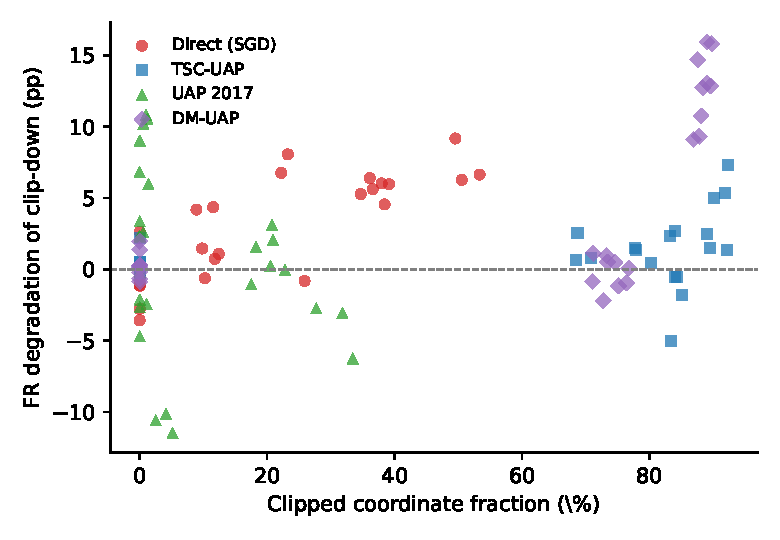
\includegraphics[width=.72\linewidth]{figs/clipfrac_scatter.pdf}
\caption{Clip-down FR change relative to per-$\epsilon$ retraining
(positive = worse than retraining), vs.\ clipped coordinate fraction
(one point per surrogate $\times$ seed $\times$ budget; at the largest budget
nothing is clipped, so those points sit at $x{=}0$ with $y$ equal to
run-to-run noise).
Points at the same $x$-position with wildly different $y$-values (e.g.,
TSC vs.\ DM-UAP at ${\sim}90\%$) show that truncation amount does not
determine damage; direction quality does. Scale-up (ours) does not appear:
it truncates no coordinate at any budget ($\max_i|\delta_i|=\epsilon$ after
rescaling), so it has no position on the $x$-axis; Figure~\ref{fig:deploy}
compares it head-to-head with clip-down.}
\label{fig:clipfrac}
\end{figure*}
% AUTO-GENERATED by make_tables.py -- DO NOT EDIT BY HAND
\begin{table*}[t]
\centering
\caption{ImageNet clip-down counterfactual: paired difference $\Delta$ (pp) of training once at $\epsilon_{\max}{=}0.3$ and clipping down, vs.\ per-$\epsilon$ retraining (upper block) and vs.\ scale-up (lower block; one training at $\epsilon_w{=}0.05$). $n{=}9$ paired runs; negative $\Delta$ favours the alternative. t: paired $t$-statistic. Entries with $|\Delta|\lesssim1.2$\,pp fall inside the cross-job reproducibility floor (Sec.~\ref{sec:limits}) and are read as ties; the mechanism claim rests on the between-optimizer contrast, not on any single small entry.}
\label{tab:clipdown}
\small
\begin{tabular}{llccc}
\toprule
Optimizer & Comparison & $\epsilon{=}0.1$ & $\epsilon{=}0.2$ & $\epsilon{=}0.3$ \\
\midrule
Direct ($\epsilon$-per-run) (clip-down) & vs.\ per-$\epsilon$ & -6.2 (-14.6) & -2.8 (-2.6) & +0.9 (+1.6) \\
TSC-UAP~\cite{huang2024texture} (clip-down) & vs.\ per-$\epsilon$ & -1.7 (-1.4) & -1.3 (-3.7) & -0.4 (-1.7) \\
UAP~\cite{moosavi2017universal} (clip-down) & vs.\ per-$\epsilon$ & +0.7 (+0.7) & -0.6 (-0.2) & -1.6 (-1.1) \\
DM-UAP~\cite{zhang2025dmuap} (clip-down) & vs.\ per-$\epsilon$ & -12.7 (-14.9) & +0.2 (+0.6) & -0.3 (-0.9) \\
\midrule
Direct ($\epsilon$-per-run) (clip-down) & vs.\ scale-up & -13.8 (-33.2) & -22.0 (-9.2) & -25.7 (-6.1) \\
TSC-UAP~\cite{huang2024texture} (clip-down) & vs.\ scale-up & -1.5 (-0.8) & -1.2 (-1.4) & -0.5 (-2.2) \\
\bottomrule
\end{tabular}
\end{table*}


Figure~\ref{fig:deploy} places the two budget-agnostic deployment strategies
in one plane, both trained once and evaluated against the same per-$\epsilon$
retraining reference. On the undersaturated SGD optimizer, clip-down is worse
than retraining at $\eps{=}0.1$ and $0.2$ ($-6.2$/$-2.8$\,pp, Table~\ref{tab:clipdown})
and only statistically tied at $\eps{=}0.3$ ($+0.9$\,pp, $t{=}1.6$), whereas
scale-up is better at every budget (by
$7.6$/$19.2$/$26.6$\,pp at $\epsilon{=}0.1/0.2/0.3$); on the well-structured
TSC optimizer the two strategies are statistically indistinguishable from
retraining. Scale-up is the only deployment strategy that dominates
retraining, and it does so with the same single training run as clip-down.
\begin{figure*}[t]
\centering
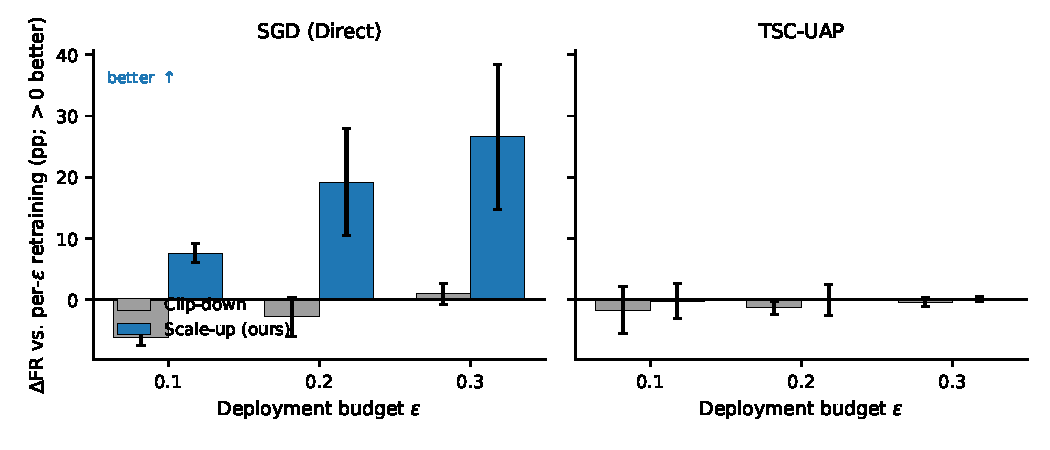
\includegraphics[width=.85\linewidth]{figs/deploy_vs_retrain.pdf}
\caption{$\Delta$FR of each budget-agnostic deployment strategy relative to
per-$\epsilon$ retraining (mean $\pm$ sd over $3$ surrogates $\times$ $3$
seeds; positive = higher fooling rate = better than retraining, matching the
$\Delta$ convention of Table~\ref{tab:clipdown}). Both strategies use a single
training run to cover all three budgets, versus three retraining runs for
the reference. On the undersaturated optimizer (left), scale-up (ours)
dominates clip-down at every budget and is the only strategy that beats
retraining; on the well-structured optimizer (right), both match retraining.}
\label{fig:deploy}
\end{figure*}

\subsection{Warm-start sensitivity and budget coverage}
Table~\ref{tab:epsw} varies the warm-start budget $\epsilon_w$. For the SGD
optimizer, $\epsilon_w\in\{0.02,0.05\}$ agree within $0.8$\,pp, and both beat
$\epsilon_w{=}0.1$ ($\sat_w{=}0.53$) by $5$--$10$\,pp---the warm-start run then
inherits exactly the failure Mechanism~1 describes. TSC-UAP is insensitive
between $\epsilon_w{=}0.05$ and $0.1$ ($\le1.8$\,pp) but loses up to $13$\,pp at
$\epsilon_w{=}0.02$, where the radius is too small for the texture objective to
leave a well-formed direction. The practical rule is therefore two-sided: the
warm-start budget must saturate \emph{and} be large enough to train a
structured direction---$0.05$ satisfies both for every optimizer we test.
Table~\ref{tab:bsweep} extends the
coverage sweep to $B{=}6$ budgets: scale-up (one run) dominates per-$\eps$
retraining ($B$ runs) at every budget, with the gap growing from $+27$ to
$+41$\,pp---supporting the linear-in-$B$ savings account of
\S\ref{sec:exp} with direct evidence.
% AUTO-GENERATED by make_tables.py -- DO NOT EDIT
\begin{table*}[t]\centering\small
\caption{Warm-start budget sensitivity (ResNet-50 surrogate, black-box mean over 3 seeds). The choice of $\epsilon_w$ matters only when the warm-start budget itself enters the undersaturated training regime ($\epsilon_w{=}0.1$, $\sat_w{=}0.53$); any sufficiently small $\epsilon_w$ works.}
\label{tab:epsw}
\begin{tabular}{llcccc}\toprule
Optimizer & $\epsilon_w$ & $\sat_w$ & $\epsilon{=}0.1$ & $0.2$ & $0.3$ \\
\midrule
direct & 0.02 & 0.99 & 0.591 & 0.846 & 0.959 \\
direct & 0.05 & 0.87 & 0.583 & 0.839 & 0.952 \\
direct & 0.1 & 0.53 & 0.485 & 0.756 & 0.898 \\
\midrule
tsc & 0.02 & 0.99 & 0.695 & 0.881 & 0.973 \\
tsc & 0.05 & 0.97 & 0.829 & 0.940 & 0.991 \\
tsc & 0.1 & 0.93 & 0.811 & 0.940 & 0.994 \\
\bottomrule\end{tabular}\end{table*}
% AUTO-GENERATED by make_tables.py -- DO NOT EDIT
\begin{table}[t]\centering\small
\caption{Budget-coverage sweep ($B{=}6$ budgets, ResNet-50, black-box mean over 3 seeds). Scale-up (one training run at $\epsilon_w{=}0.05$) dominates per-$\epsilon$ retraining (six runs) at every budget, with the gap growing in $\epsilon$; covering six budgets costs $1/6$ the training compute.}
\label{tab:bsweep}
\begin{tabular}{lcccccc}\toprule
$\epsilon$ & 0.05 & 0.1 & 0.15 & 0.2 & 0.25 & 0.3 \\
\midrule
Scale-up (1 run) & 0.640 & 0.819 & 0.868 & 0.922 & 0.967 & 0.989 \\
Per-$\epsilon$ ($B$ runs) & 0.366 & 0.490 & 0.537 & 0.575 & 0.577 & 0.575 \\
\midrule
$\Delta$ & +0.274 & +0.329 & +0.332 & +0.348 & +0.390 & +0.414 \\
\bottomrule\end{tabular}\end{table}

\subsection{Zero-optimization directions: is budget-agnostic deployment trivial?}
A natural objection: any fixed direction is budget-agnostic by construction,
so why train at all? The singular-vector UAP of~\cite{khrulkov2018art} is the
sharpest version of this objection---from as few as 64 images, with
\emph{zero} optimization, it extracts the top right singular vector of the
layer Jacobian and can be scaled exactly to any $\eps$. We implement it
faithfully (power iteration through forward-mode JVPs with the ImageNet
normalization inside the Jacobian, sign-aligned averaging over images,
$k{\in}\{64,200\}$, two depths; all runs converge, residual ${<}10^{-4}$) and
evaluate it under the identical protocol (Table~\ref{tab:svd}). The objection
fails decisively: the best SVD configuration reaches only
$25.6$/$28.1$/$30.7$\% black-box at $\eps{=}0.1/0.2/0.3$, against
$57.7$/$83.5$/$95.1$\% for scale-up---paired differences of
$+32$/$+55$/$+65$\,pp ($t{\ge}85$, $n{=}3$ seeds)---and even per-$\eps$
direct retraining beats it by $20$--$28$\,pp. The mechanism contrast is
equally stark: the SVD direction has $\sat<10^{-5}$ (a dense direction with
essentially no coordinates on the $L_\infty$ boundary, versus $0.03$--$0.93$
boundary occupancy for direct training across our sweeps), so the advantage is
not explained by boundary saturation either. Budget-agnostic deployment is therefore
necessary but not sufficient: the optimization-derived direction, not the
scaling convention, carries the transfer advantage.
% AUTO-GENERATED by make_tables.py -- DO NOT EDIT BY HAND
\begin{table*}[t]
\centering
\caption{SVD direction baseline (ResNet-50 surrogate, black-box mean over the 4 remaining targets, 3 seeds). The singular-vector direction of~\cite{khrulkov2018art} uses no optimization at all ($k{\in}\{64,200\}$ images, top right singular vector of the layer Jacobian; rows ``layer2''/``layer4'' denote the layer whose Jacobian is decomposed) and is budget-agnostic by construction ($\delta(\epsilon){=}\epsilon\,\hat v$, exact at every $\epsilon$). $\Delta$: paired scale-up $-$ SVD difference (pp) for the best SVD configuration; t: paired $t$-statistic over 3 seeds.}
\label{tab:svd}
\small
\begin{tabular}{lcccc}
\toprule
Method & Opt.\ runs & $\epsilon{=}0.1$ & $\epsilon{=}0.2$ & $\epsilon{=}0.3$ \\
\midrule
Scale-up (SGD) & 1 & 57.7 & 83.5 & 95.1 \\
Direct & 3 & 48.4 & 56.3 & 57.9 \\
\midrule
SVD ($k{=}200$, layer2) (best) & 0 & 25.6 & 28.1 & 30.7 \\
SVD ($k{=}200$, layer4) & 0 & 25.4 & 27.3 & 29.6 \\
SVD ($k{=}64$, layer2) & 0 & 25.1 & 26.7 & 28.1 \\
SVD ($k{=}64$, layer4) & 0 & 24.8 & 26.0 & 27.3 \\
\midrule
$\Delta$: Scale-up $-$ SVD (best) & -- & +32.1 (+85.4) & +55.4 (+88.4) & +64.5 (+107.7) \\
\bottomrule
\end{tabular}
\end{table*}


\subsection{Cross-dataset control (CIFAR-10, FR-ceiling-bound regime)}
Table~\ref{tab:cifar}. A pre-registered falsification test: on CIFAR-10 all
four optimizers, at all three budgets, and under all three deployment
strategies converge to the same irreducible ceiling
($\mathrm{FR}\approx 91.1\pm0.1\%$ black-box; the $\approx$9\% remainder is
never fooled). The paired advantage of scale-up over per-$\eps$ retraining is
$|\Delta|\le 0.07$\,pp at the aggregate level over all $24$
method$\times$budget$\times$strategy comparisons ($n{=}9$ runs
each; individual runs spread by at most $0.3$\,pp)---more than two orders of
magnitude smaller than on ImageNet. Notably, the regime is not fully
saturated: direct training still shows a genuine undersaturation signature
($\sat$ declining $0.56\to0.39$ with $\eps$, while scaled perturbations keep
$\sat\equiv\sat(\eps_w)=0.62$ constant, empirically confirming the
shape-preservation property of \S\ref{sec:method}). The advantage is absent
anyway because the FR ceiling binds. This yields a clean decomposition the
two-factor criterion requires: \emph{an undersaturation gap alone is not
sufficient; the ceiling must also be unbinding}---consistent with the three
ceiling-hit exceptions in the $r{=}0.807$ correlation. The conditionality of
our claims survives its strongest attempted falsification.
% AUTO-GENERATED by make_tables.py -- DO NOT EDIT BY HAND
\begin{table*}[t]
\centering
\caption{CIFAR-10 control (FR-ceiling-bound regime): black-box fooling rate (\%), same protocol as the ImageNet experiments (Table~\ref{tab:protocol}). Every method, budget, and deployment strategy converges to the same irreducible ceiling ($\approx$91\%), so the three strategies coincide---the advantage is conditioned on the ceiling being unbinding.}
\label{tab:cifar}
\small
\begin{tabular}{lcccc}
\toprule
Method & $\epsilon$ & per-$\epsilon$ & clip-down & scale-up \\
\midrule
Direct ($\epsilon$-per-run) & 0.1 & 91.1 & 91.1 & 91.1 \\
 & 0.2 & 91.1 & 91.1 & 91.2 \\
 & 0.3 & 91.1 & 91.1 & 91.1 \\
\midrule
DM-UAP~\cite{zhang2025dmuap} & 0.1 & 91.1 & 91.1 & 91.1 \\
 & 0.2 & 91.1 & 91.2 & 91.1 \\
 & 0.3 & 91.2 & 91.2 & 91.1 \\
\midrule
TSC-UAP~\cite{huang2024texture} & 0.1 & 91.2 & 91.1 & 91.1 \\
 & 0.2 & 91.1 & 91.2 & 91.1 \\
 & 0.3 & 91.2 & 91.2 & 91.1 \\
\midrule
UAP~\cite{moosavi2017universal} & 0.1 & 91.1 & 91.1 & 91.1 \\
 & 0.2 & 91.1 & 91.1 & 91.2 \\
 & 0.3 & 91.2 & 91.2 & 91.1 \\
\bottomrule
\end{tabular}
\end{table*}


\subsection{Cost accounting}
Table~\ref{tab:cost} reports measured GPU-seconds. Covering all three budgets
takes $78$\,s with scale-up versus $231$\,s for per-budget SGD retraining
($2.9\times$), $232$\,s for TSC ($3.0\times$), and $764$\,s for DM-UAP
($9.7\times$)---and even DM-UAP's single run costs $3.3\times$ a scale-up run
(measured wall-clock, Table~\ref{tab:cost}). The savings grow linearly in the
number of deployed budgets $B$; Table~\ref{tab:bsweep} verifies this directly
at $B{=}6$ ($83\%$ saved, with scale-up also stronger at every budget).
% AUTO-GENERATED by make_tables.py -- DO NOT EDIT BY HAND
\begin{table}[t]
\centering
\caption{Measured training compute (GPU-seconds, mean $\pm$ sd over 9 runs, i.e., 3 surrogates $\times$ 3 seeds; the spread is dominated by architecture cost differences, e.g., ViT trains $\sim$4$\times$ slower than ResNet-50) to cover all three budgets $\epsilon\in\{0.1,0.2,0.3\}$. Scale-up trains once at $\epsilon_w{=}0.05$ and rescales; baselines train per budget (three runs). DM-UAP additionally uses $3.3\times$ more compute \emph{per run} by its official settings. The two cheaper entries are not FR-comparable to the scale-up instance we quote: UAP~\cite{moosavi2017universal} ($1.8\times$) trails it by $26.7$--$34.2$\,pp and per-$\epsilon$ SGD retraining ($2.9\times$) by $22.7$--$29.3$\,pp at every budget, so the $3.0\times$--$9.7\times$ range is restricted to FR-competitive baselines.}
\label{tab:cost}
\small
\begin{tabular}{lccr}
\toprule
Method & Runs & GPU-s (total) & Rel.\ scale-up \\
\midrule
Scale-up (SGD) & 1 & 78 $\pm$ 48 & 1.0$\times$ \\
Scale-up (TSC) & 1 & 77 $\pm$ 49 & 1.0$\times$ \\
Direct ($\epsilon$-per-run)$^{3}$ & 3 & 231 $\pm$ 146 & 2.9$\times$ \\
UAP~\cite{moosavi2017universal}$^{3}$ & 3 & 145 $\pm$ 94 & 1.8$\times$ \\
TSC-UAP~\cite{huang2024texture}$^{3}$ & 3 & 232 $\pm$ 146 & 3.0$\times$ \\
DM-UAP~\cite{zhang2025dmuap}$^{3}$ & 3 & 764 $\pm$ 471 & 9.7$\times$ \\
\bottomrule
\end{tabular}
\\
\footnotesize $^{3}$: three per-budget runs; totals include all three. DM-UAP per-run wall-clock is $3.3\times$ scale-up's single run.
\end{table}


\subsection{Cross-architecture transfer (ViT)}
Including ViT-B/16 in the surrogate and target pool, the scale-up advantage
persists in all three blocks of the cross-architecture matrix (CNN$\times$CNN,
CNN$\to$ViT, ViT$\to$CNN) at all budgets. Two asymmetries are worth noting.
First, ViT as \emph{surrogate} benefits most: white-box FR at $\eps{=}0.2$
reaches $0.952$ vs.\ $0.607$ for direct training ($+34.5$\,pp). Second,
CNN$\to$ViT absolute transfer is inherently weak (best FR $\le 0.87$ among the
SGD-family arms of this run; the texture-guided instance reaches $0.97$ in the
main grid, Table~\ref{tab:permodel}), but
scale-up still recovers $81$--$94\%$ of the achievable ceiling---e.g.,
$94.1\%$ ceiling attainment vs.\ $62.0\%$ for direct at $\eps{=}0.3$---while
ViT$\to$CNN transfers strongly ($0.73$--$0.99$). These gains, too, are
measured against the default-lr direct baseline and shrink or vanish against
a tuned lr$=0.05$ baseline (\S\ref{sec:limits}, item 4).

\subsection{Modern evaluation targets (ConvNeXt-T, Swin-T, EfficientNet-B0)}
The original target pool is 4 CNNs (2015--2019) plus one ViT; a reviewer may
wonder whether the conclusions depend on target vintage. We add three
2020+ architectures---ConvNeXt-T, Swin-T, and EfficientNet-B0---to the
evaluation pool and retrain all four headline methods under the identical
protocol (ResNet-50 surrogate, 3 seeds; Table~\ref{tab:p2}). Both
pre-registered predictions hold. (i)~The scale-up advantage over per-$\eps$
retraining is preserved, and grows: on the new-target mean the paired
advantage is $+7.6/+31.7/+49.9$pp at $\eps{=}0.1/0.2/0.3$
(all $9/9$ seed--target pairs positive at every budget), because the undersaturation collapse
of direct training is \emph{more severe} on the newer targets (new-mean
34--43\% vs.\ 49--59\% on the original pool). (ii)~No modern-architecture
immunity appears: absolute transferable FR on the new targets spans the same
range as the original pool, and the TSC-family budget-agnostic deployment
again matches its per-budget retraining counterpart
($|\Delta|\leq0.9$pp, all n.s.). As a protocol check, the retrained
old-pool measurements reproduce the ResNet-50 rows of
Table~\ref{tab:main-imagenet} within $0.7$pp at every budget.
% AUTO-GENERATED by make_tables.py -- DO NOT EDIT BY HAND
\begin{table*}[t]
\centering
\caption{Modern-architecture evaluation targets (ResNet-50 surrogate, 3 seeds, 200-shot protocol of Table~\ref{tab:protocol}). Three 2020+ targets are added to the pool: ConvNeXt-T, Swin-T, EfficientNet-B0; all methods are retrained under the identical protocol (fresh runs; the repeated old-pool measurements reproduce the ResNet-50 rows of Table~\ref{tab:main-imagenet} within 0.7pp). ``New-mean'': mean over the 3 new targets. $\Delta$ rows: paired difference (pp) on the new-target mean per budget, with paired $t$ over 3 seeds.}
\label{tab:p2}
\small
\begin{tabular}{llcccc}
\toprule
Method & $\eps$ & ConvNeXt-T & Swin-T & EffNet-B0 & New-mean \\
\midrule
Scale-up (SGD) & 0.1 & 34.2 & 33.0 & 58.7 & 42.0 \\
Scale-up (SGD) & 0.2 & 66.0 & 60.8 & 90.2 & 72.4 \\
Scale-up (SGD) & 0.3 & 90.8 & 88.1 & 98.7 & 92.5 \\
\midrule
Scale-up (TSC) & 0.1 & 86.6 & 51.7 & 95.8 & 78.0 \\
Scale-up (TSC) & 0.2 & 99.1 & 88.0 & 99.7 & 95.6 \\
Scale-up (TSC) & 0.3 & 99.9 & 99.1 & 99.8 & 99.6 \\
\midrule
Direct & 0.1 & 29.5 & 29.0 & 44.6 & 34.4 \\
Direct & 0.2 & 34.9 & 34.6 & 52.3 & 40.6 \\
Direct & 0.3 & 36.1 & 37.5 & 54.2 & 42.6 \\
\midrule
TSC-UAP & 0.1 & 87.9 & 50.2 & 93.4 & 77.2 \\
TSC-UAP & 0.2 & 99.3 & 90.2 & 99.6 & 96.4 \\
TSC-UAP & 0.3 & 99.8 & 99.4 & 99.8 & 99.7 \\
$\Delta$: Scale-up (SGD) $-$ Direct & 0.1 & & & & +7.6 (+13.3) \\
$\Delta$: Scale-up (SGD) $-$ Direct & 0.2 & & & & +31.7 (+89.2) \\
$\Delta$: Scale-up (SGD) $-$ Direct & 0.3 & & & & +49.9 (+62.3) \\
$\Delta$: Scale-up (TSC) $-$ TSC-UAP & 0.1 & & & & +0.9 (+2.8) \\
$\Delta$: Scale-up (TSC) $-$ TSC-UAP & 0.2 & & & & -0.8 (-0.9) \\
$\Delta$: Scale-up (TSC) $-$ TSC-UAP & 0.3 & & & & -0.1 (-0.4) \\
\bottomrule
\end{tabular}
\end{table*}


% ----------------------------------------------------------------------------
\section{Limitations and Scope}\label{sec:limits}
Six boundaries, stated plainly (reviewers will probe each):
\begin{enumerate}
  \item \textbf{No accuracy advantage over saturated SOTA}: at $\eps{=}0.1$
        DM-UAP leads; our claim is the budget-coverage compute account, not
        single-point accuracy;
  \item \textbf{Advantage conditioned on undersaturation with an unbinding
        ceiling}: in ceiling-bound regimes (CIFAR-10) or for well-structured
        optimizers (TSC-type) the advantage vanishes---claims must be
        conditioned;
  \item \textbf{Surrogate dependence}: the effect is determined by the
        surrogate family, not the target (vgg/mobilenet surrogates hit the
        FR ceiling);
  \item \textbf{Loses at a single budget to free hyperparameter tuning}:
        direct training with lr${=}0.05$ is uniformly stronger at one budget;
        the primitive pays off only in multi-budget deployment;
  \item \textbf{Norm scope}: all headline results are $L_\infty$. An
        $L_2$ spot-check (Table~\ref{tab:l2}) finds direct-$L_2$ and
        scale-up-$L_2$ at parity at every tested radius ($|\Delta|\le1$\,pp),
        i.e., the $L_\infty$-specific failure--rescue contrast does not
        transfer to $L_2$ at these small budgets; norm-general claims
        therefore require further study.
  \item \textbf{Cross-job reproducibility}: recomputing the same nominal cell
        in a different job moves it by up to $1.2$\,pp. The cause is not seed
        noise (seeds are shared within a job) but surrogate re-instantiation
        and single-run target noise, so the floor applies across artifacts and
        not within one. We therefore interpret no difference below $1.2$\,pp,
        which makes the sub-floor entries of Table~\ref{tab:clipdown} ties; the
        same-process control of Table~\ref{tab:cifar}, which shares one
        evaluation pass, is unaffected.
\end{enumerate}
% AUTO-GENERATED by make_tables.py -- DO NOT EDIT
\begin{table}[t]\centering\small
\caption{$L_2$ spot-check (ResNet-50, black-box mean over 3 seeds, global $\|\delta\|_2 \le \epsilon$ projection). Direct-$L_2$ and scale-up-$L_2$ are at parity at every budget ($|\Delta| \le 1$\,pp), consistent with the $L_\infty$ finding that under $L_2$ few-shot training is not budget-coupled-degraded at these small radii.}
\label{tab:l2}
\begin{tabular}{lccc}\toprule
$\|\delta\|_2 \le$ & 5 & 10 & 20 \\
\midrule
Direct-$L_2$ & 0.268 & 0.310 & 0.417 \\
Scale-up-$L_2$ & 0.267 & 0.310 & 0.427 \\
$\Delta$ & -0.001 & +0.000 & +0.010 \\
\bottomrule\end{tabular}\end{table}

% ----------------------------------------------------------------------------
\section{Conclusion}
Deployment--training budget decoupling is a previously unexamined degree of
freedom in UAP practice. Scale-up realizes it as a one-training-for-any-budget
primitive whose applicability is precisely characterized by two mechanistic
quantities and stress-tested by a ceiling-bound-regime control. We equally
report the negative result: at a single budget the primitive does not beat a
tuned direct baseline.

% ----------------------------------------------------------------------------
\begin{thebibliography}{99}

\bibitem{moosavi2017universal}
S.-M.~Moosavi-Dezfooli, A.~Fawzi, O.~Fawzi, and P.~Frossard.
\newblock Universal adversarial perturbations.
\newblock In \emph{CVPR}, 2017.

\bibitem{szegedy2014intriguing}
C.~Szegedy, W.~Zaremba, I.~Sutskever, J.~Bruna, D.~Erhan, I.~Goodfellow, and
  R.~Fergus.
\newblock Intriguing properties of neural networks.
\newblock In \emph{ICLR}, 2014.

\bibitem{goodfellow2015fgsm}
I.~J. Goodfellow, J.~Shlens, and C.~Szegedy.
\newblock Explaining and harnessing adversarial examples.
\newblock In \emph{ICLR}, 2015.

\bibitem{carlini2017cw}
N.~Carlini and D.~Wagner.
\newblock Towards evaluating the robustness of neural networks.
\newblock In \emph{IEEE Symposium on Security and Privacy}, 2017.

\bibitem{madry2018pgd}
A.~Madry, A.~Makelov, L.~Schmidt, D.~Tsipras, and A.~Vladu.
\newblock Towards deep learning models resistant to adversarial attacks.
\newblock In \emph{ICLR}, 2018.

\bibitem{papernot2017practical}
N.~Papernot, P.~McDaniel, I.~Goodfellow, S.~Jha, Z.~B. Celik, and A.~Swami.
\newblock Practical black-box attacks against machine learning.
\newblock In \emph{AsiaCCS}, 2017.

\bibitem{liu2017ndss}
Y.~Liu, X.~Chen, C.~Liu, and D.~Song.
\newblock Delving into transferable adversarial examples and black-box
  attacks.
\newblock In \emph{ICLR}, 2017.

\bibitem{evtimov2018semantic}
K.~Eykholt, I.~Evtimov, E.~Fernandes, B.~Li, A.~Rahmati, C.~Xiao,
  A.~Prakash, T.~Kohno, and D.~Song.
\newblock Robust physical-world attacks on deep learning visual
  classification.
\newblock In \emph{CVPR}, pages 1625--1634, 2018.

\bibitem{khrulkov2018art}
V.~Khrulkov and I.~Oseledets.
\newblock Art of singular vectors and universal adversarial perturbations.
\newblock In \emph{CVPR}, pages 8562--8570, 2018.

\bibitem{mopuri2017ffa}
K.~R. Mopuri, U.~Garg, and R.~V. Babu.
\newblock Fast feature fool: A data independent approach to universal
  adversarial perturbations.
\newblock In \emph{BMVC}, 2017.

\bibitem{mopuri2019generalizable}
K.~R. Mopuri, A.~Ganeshan, and R.~V. Babu.
\newblock Generalizable data-free objective for crafting universal
  adversarial perturbations.
\newblock \emph{IEEE Transactions on Pattern Analysis and Machine
  Intelligence}, 41(10):2452--2465, 2019.

\bibitem{poursaeed2018generative}
O.~Poursaeed, I.~Katsman, B.~Gao, and S.~Belongie.
\newblock Generative adversarial perturbations.
\newblock In \emph{CVPR}, pages 4422--4431, 2018.

\bibitem{wang2024fduap}
D.~Wang, W.~Yao, T.~Jiang, and X.~Chen.
\newblock Improving transferability of universal adversarial perturbation
  with feature disruption.
\newblock \emph{IEEE Transactions on Image Processing}, 33:722--737, 2024.

\bibitem{weng2024metauap}
J.~Weng, Z.~Luo, D.~Lin, and S.~Li.
\newblock Learning transferable targeted universal adversarial perturbations
  by sequential meta-learning.
\newblock \emph{Computers \& Security}, 137:103584, 2024.

\bibitem{weng2024survey}
J.~Weng, Z.~Luo, D.~Lin, and S.~Li.
\newblock Comparative evaluation of recent universal adversarial
  perturbations in image classification.
\newblock \emph{Computers \& Security}, 136:103576, 2024.

\bibitem{huang2024texture}
Y.~Huang, Q.~Guo, F.~Juefei-Xu, M.~Hu, X.~Jia, X.~Cao, G.~Pu, and Y.~Liu.
\newblock Texture re-scalable universal adversarial perturbation.
\newblock \emph{IEEE Transactions on Information Forensics and Security},
  19:8291--8305, 2024.

\bibitem{zhang2025dmuap}
Y.~Zhang, Y.~Xu, J.~Shi, L.~Y. Zhang, S.~Hu, M.~Li, and Y.~Zhang.
\newblock Improving generalization of universal adversarial perturbation via
  dynamic maximin optimization.
\newblock In \emph{AAAI}, pages 10293--10301, 2025.

\bibitem{akhtar2018defense}
N.~Akhtar, J.~Liu, and A.~Mian.
\newblock Defense against universal adversarial perturbations.
\newblock In \emph{CVPR}, 2018.

\bibitem{shafahi2019universal}
A.~Shafahi, M.~Najibi, Z.~Xu, J.~Dickerson, L.~S. Davis, and T.~Goldstein.
\newblock Universal adversarial training.
\newblock In \emph{AAAI}, volume 34, pages 5636--5643, 2020.

\bibitem{athalye2018obfuscated}
A.~Athalye, N.~Carlini, and D.~Wagner.
\newblock Obfuscated gradients give a false sense of security: Circumventing
  defenses to adversarial examples.
\newblock In \emph{ICML}, 2018.

\bibitem{croce2021robustbench}
F.~Croce, M.~Andriushchenko, V.~Sehwag, N.~Debenedetti, N.~Flammarion,
  M.~Chiang, P.~Mittal, and M.~Hein.
\newblock RobustBench: A standardized adversarial robustness benchmark.
\newblock In \emph{NeurIPS Datasets and Benchmarks Track}, 2021.

\bibitem{he2016resnet}
K.~He, X.~Zhang, S.~Ren, and J.~Sun.
\newblock Deep residual learning for image recognition.
\newblock In \emph{CVPR}, 2016.

\bibitem{simonyan2015vgg}
K.~Simonyan and A.~Zisserman.
\newblock Very deep convolutional networks for large-scale image recognition.
\newblock In \emph{ICLR}, 2015.

\bibitem{howard2018mobilenet}
M.~Sandler, A.~Howard, M.~Zhu, A.~Zhmoginov, and L.-C. Chen.
\newblock MobileNetV2: Inverted residuals and linear bottlenecks.
\newblock In \emph{CVPR}, 2018.

\bibitem{dosovitskiy2021vit}
A.~Dosovitskiy, L.~Beyer, A.~Kolesnikov, et~al.
\newblock An image is worth 16x16 words: Transformers for image recognition
  at scale.
\newblock In \emph{ICLR}, 2021.

\bibitem{krizhevsky2009cifar}
A.~Krizhevsky.
\newblock Learning multiple layers of features from tiny images.
\newblock Technical report, University of Toronto, 2009.

\bibitem{huang2017densenet}
G.~Huang, Z.~Liu, L.~van~der Maaten, and K.~Q. Weinberger.
\newblock Densely connected convolutional networks.
\newblock In \emph{CVPR}, 2017.

\bibitem{ma2018shufflenet}
N.~Ma, X.~Zhang, H.-T. Zheng, and J.~Sun.
\newblock ShuffleNet V2: Practical guidelines for efficient CNN
  architecture design.
\newblock In \emph{ECCV}, 2018.

\end{thebibliography}

\appendix
\section{Proofs of Scale-up Properties}\label{app:proof}
\textbf{Property (i), shape preservation.}
Let $\|\delta_w\|_\infty \le \eps_w$ and $\delta(\eps) =
(\eps/\eps_w)\delta_w$ with $\eps \ge \eps_w$. For every coordinate $i$,
$|\delta(\eps)_i| = (\eps/\eps_w)|\delta_{w,i}| \le (\eps/\eps_w)\eps_w =
\eps$, so $\|\delta(\eps)\|_\infty \le \eps$; and
$|\delta(\eps)_i| = \eps \iff |\delta_{w,i}| = \eps_w$. Hence the boundary
occupation of each coordinate is unchanged:
$\mathrm{sat}(\delta(\eps);\eps) =
\mathrm{sat}(\delta_w;\eps_w)$, and more generally the whole indicator
profile $(\mathbf{1}[|\delta_{w,i}|{=}\eps_w])_i$ is invariant. This is the
invariance observed empirically in the CIFAR-10 control.

\textbf{Property (ii), zero loss (invertibility).}
Radial rescaling $r \mapsto (\eps/\eps_w) r$ is a bijection between the
$L_\infty$ balls $B_{\eps_w}$ and $B_{\eps}$ (its inverse is scaling by
$\eps_w/\eps$), so no information is discarded. In contrast, the clip-down
map $\Pi_{B_\eps}(\cdot)$ restricted to coordinates in the shell
$\{\eps < |\delta_i| \le \eps_{\max}\}$ is many-to-one (all shell values
collapse to $\pm\eps$), hence non-invertible: the discarded shell magnitude
is unrecoverable. Whether the preserved direction suffices for a given
target is an empirical question---Property (ii) concerns the map's geometry,
not FR, which is not scale-covariant under a nonlinear $f$.

\textbf{Proof of Proposition 1 (saturation collapse).}
First suppose no noise ($\sigma = 0$). By induction, the projected update
keeps coordinate $i$ monotone: $\delta_i^t = \mathrm{sign}(\mu_i)\cdot
\min(\eta t \mu_i, \eps)$ for all $t$ (base $t{=}0$ trivial; the projection
clamps at $\eps$ exactly when $\eta t \mu_i \ge \eps$, after which the
iterate remains at the boundary because the update points outward). Hence
at $t = T$, coordinate $i$ is saturated iff $\eta T \mu_i \ge \eps$, i.e.,
$\mu_i \ge \eps/(\eta T)$, giving
$\sat(\eps) = \Pr[\mu_i \ge \eps/(\eta T)] = 1 - F_\mu(\eps/(\eta T))$.
This is non-increasing in $\eps$ and tends to
$1 - F_\mu(\infty) = 0$ whenever $F_\mu$ has full support on
$(0,\infty)$. With noise, coordinate $i$ saturates iff
$\eta (T\mu_i + \sigma\textstyle\sum_t \xi_i^t) \ge \eps$; since
$\sum_t \xi_i^t / \sqrt{T}$ is asymptotically $\mathcal{N}(0,1)$, the
per-coordinate threshold becomes $\eps - \eta\sigma\sqrt{T} z$ with
$z \sim \mathcal{N}(0,1)$ drawn once per coordinate, and
$\sat(\eps) = \mathbb{E}_z\big[1 - F_\mu((\eps -
\eta\sigma\sqrt{T}z)_+ / (\eta T))\big]$, the drift-noise curve in
Figure~\ref{fig:theory}. (For adversarially aligned $\xi$ the bound holds
whp. by sub-Gaussian concentration; we do not need that refinement.)
\hfill\openbox

\textbf{Proof of Proposition 3 (profile distortion).}
Scale-up: for any coordinates $i, j$ with $\delta_{w,i}, \delta_{w,j} \neq
0$, $\delta_i(\eps)/\delta_j(\eps) = \delta_{w,i}/\delta_{w,j}$ for every
$\eps$, so the full ratio structure (direction, up to positive scaling) is
preserved exactly. Clip-down: if coordinate $i$ is clipped, then
$|\delta_i| > \eps$ and after projection $|\Pi(\delta)_i| = \eps$; thus for
any two clipped coordinates $i, j$ (with the same sign),
$\Pi(\delta)_i / \Pi(\delta)_j = 1$ regardless of their original ratio,
which may have been arbitrarily large. The ratio structure on the clipped
set is therefore collapsed to a constant, and the fraction of coordinates
affected is exactly the clipped mass $\mathrm{clip\text{-}frac}$; the
interior (unclipped) coordinates are untouched, so their relative weight in
the perturbation grows as the clipped set grows. This is the sense in which
truncation destroys directional information in proportion to the clipped
mass, while rescaling destroys none.
\hfill\openbox

\section{Hyperparameters and Protocol Details}\label{app:hyper}
\textbf{Common.} Training pool $k{=}200$ (split seed 100), evaluation
2{,}000 held-out images (split seed 42), pixel range $[0,1]$, $L_\infty$
threat model. All evaluations run in \texttt{eval()} mode, where the batch
size provably does not affect FR (batch-norm uses running statistics); we
confirmed this empirically before the main runs.
\textbf{SGD direct / scale-up.} 200 steps, lr $0.01$ (the tuned-lr ablation
uses lr $0.05$), batch 128.
\textbf{UAP'17.} 200 steps, lr $0.02$, batch 128.
\textbf{TSC-UAP.} Texture scale $\alpha{=}4$, 200 steps, lr $0.01$,
batch 128, followed by the official assembly step.
\textbf{DM-UAP.} Official implementation and settings: 60 outer steps,
$\theta$-steps 10, $cc{=}10$, batch 50 (ImageNet); on our hardware this costs
$3.3\times$ the wall-clock of one scale-up run (measured,
Table~\ref{tab:cost}), i.e., the comparison
deliberately favors the baseline.
\textbf{Seeds.} $42, 1342, 2342$ for UAP optimization and split sampling;
train and evaluation splits are drawn with disjoint seeds and never overlap.

\section{Full Per-Model Results}\label{app:permodel}
Table~\ref{tab:permodel} lists per-target black-box FR for selected methods
at the two extreme budgets; the complete grid (9 methods $\times$ 3 budgets
$\times$ 5 models $\times$ 9 runs) is in the released JSONs.
% AUTO-GENERATED by make_tables.py -- DO NOT EDIT BY HAND
\begin{table*}[t]
\centering
\caption{Per-target black-box fooling rate (\%) on ImageNet (mean over 3 surrogates $\times$ 3 seeds; the surrogate itself is excluded when it appears as a target). Selected methods and the two extreme budgets; full grid in the released JSONs.}
\label{tab:permodel}
\small
\begin{tabular}{llccccc}
\toprule
Method & $\epsilon$ & ResNet-50 & VGG-16-BN & ResNet-101 & MobileNet-V2 & ViT-B/16 \\
\midrule
Scale-up (TSC) & 0.1 & 87.8 & 90.1 & 85.1 & 93.3 & 39.2 \\
 & 0.3 & 99.6 & 99.8 & 99.5 & 99.8 & 97.8 \\
\midrule
Direct & 0.1 & 56.5 & 61.5 & 51.7 & 70.6 & 32.8 \\
 & 0.3 & 73.2 & 77.5 & 66.7 & 83.5 & 43.1 \\
\midrule
DM-UAP & 0.1 & 91.8 & 90.1 & 88.8 & 93.4 & 54.5 \\
 & 0.3 & 99.3 & 99.4 & 99.3 & 99.6 & 85.3 \\
\bottomrule
\end{tabular}
\end{table*}


\section{Reproducibility}\label{app:repro}
All numeric tables (Tables~\ref{tab:main-imagenet},
\ref{tab:clipdown}, \ref{tab:cifar}, \ref{tab:cost}, and
\ref{tab:permodel}) and Figure~\ref{fig:clipfrac} are generated
programmatically by a script (\texttt{make\_tables.py} and
its companion \texttt{make\_figures.py}) directly from the raw result JSONs; no
number is
transcribed by hand. The anonymous repository will contain: all training and
evaluation drivers, the vendored official DM-UAP implementation (mechanical
adaptations only), the third-party baseline implementations, and every
result JSON backing the tables. Pre-registered predictions for the CIFAR-10
control were recorded before the run was launched and are reproduced in
\S\ref{sec:exp} verbatim.

% ----------------------------------------------------------------------------
\section{Open Science}\label{app:openscience}
We fully support the Open Science policy of ACM ASIACCS.
\textbf{Artifacts.} The complete artifact is prepared and will be released
publicly upon acceptance. It contains: (i) every training and evaluation
driver (\texttt{run\_*.py}), including the few-shot UAP optimizer, the
budget-agnostic deployment procedures, the clip-down counterfactual driver,
the singular-vector baseline, and the cross-dataset and cross-architecture
controls; (ii) the vendored official implementation of the DM-UAP baseline
(mechanical adaptations only, algorithm unchanged) together with our
re-implementations of the remaining 2017--2025 baselines; (iii) all raw
result JSONs backing every table and figure of this paper; and (iv) the
table/figure generators (\texttt{make\_tables.py}, \texttt{make\_figures.py})
that reproduce every number in this paper directly from those JSONs, with no
hand transcription.
\textbf{Anonymized repository.} For double-blind review the artifact is
available at: \todo{insert anonymous.4open.science link before submission}.
\textbf{Datasets and models.} All experiments use only publicly available
datasets (ImageNet-mini, CIFAR-10) and off-the-shelf pretrained weights from
\texttt{torchvision}; no proprietary or human-subject data is involved.

% ----------------------------------------------------------------------------
\section{Ethical Considerations}\label{app:ethics}
This work studies the optimization and deployment of universal adversarial
perturbations (UAPs) against image classifiers. All experiments are conducted
offline on public datasets and public pretrained models; no real system, no
service, and no human subject is involved, and no data was collected from
users. The paper therefore raises no privacy concern and required no IRB
approval.

Like the rest of the UAP literature~\cite{moosavi2017universal}, this
research is dual-use. Its practical message is deliberately narrow and, if
anything, defensive in value: (i) it shows that a single low-budget
perturbation can be rescaled to larger budgets, which means that
\emph{defenders} who evaluate robustness only at the budgets they happen to
train against may underestimate exposure at other radii; and (ii) it
identifies two measurable quantities (\emph{saturation fraction} and
\emph{clip fraction}) plus a minimal model that predict \emph{when}
few-shot budget-coupled training fails, which supports cheap robustness
auditing. The compute saving we report ($3.0\times$--$9.7\times$, against the
FR-competitive baselines) lowers the cost
of constructing transferable perturbations, but it does not change the threat
model of existing transfer attacks: the perturbations remain
$L_\infty$-bounded, white-box-transfer, and 200-image few-shot; they are not
query-based, not physically realizable in the settings we test, and not
evaluated against any deployed defense. We release code and results to
support reproducible robustness evaluation rather than to enable misuse, and
we consider the standard responsible-disclosure process inapplicable because
no specific vulnerable system is identified.

\end{document}
